\newpage

\section{Part 3: Hidden Markov Models (HMM)}

Hidden Markov Models (HMMs) are used to detect patterns in sequences in a probabilistic way. Another way to detect patterns could be via regular expressions, but these don't capture exceptions, consensus, or higher probabilities for certain amino acids or certain sequence positions than others, etc.

\subsection{Log Odds to Score Sequences}

In section \ref{sec:substmats} we have seen that a log-odds ratio is commonly used to compute scores in amino acid and nucleotide substitution matrices. A similar log odds ratio is used to score entire sequences as well. The {\bf log odds} for a nucleotide sequence S of length L is:
\begin{equation}
\log \frac{P(S)}{0.25^L} = \log(P(S)) - L \; \log(0.25)
\end{equation}

This metric is used to scale and normalize by a random model. Scaling is important in order not to penalize longer sequences (that would otherwise get lower probability, because they get more numbers smaller than one multiplied together). Normalizing by a random model is important to highlight the real patterns from the background noise.

\subsection{Markov Chain}

Figure \ref{fig:markovchain} shows an example of Markov Chain (MC). It is a state machine with one symbol per state. After emitting the symbol, the machine transitions to one of the possible next states with a given probability.
A sequence $x = x_1, ... x_L$ can be generated from the MC state machine in this way. Each symbol $x_i$ belongs to the alphabet $\mathcal{A}$ that also defines the set of states of the state machine: $x_i \in \mathcal{A}$, e.g. $\mathcal{A} = \{ A, C, T, G \}$ for a nucleotide sequence $x$.

\begin{figure}[!htb]
\centerline{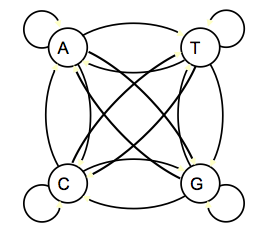
\includegraphics[width=.3\linewidth]{figs/MarkovChain-example.png}}
\caption{Example of Markov Chain}\label{fig:markovchain}
\end{figure}

The transition probability $a_{st}$ to go from state $s$ to state $t$ is:
\begin{equation}
\boxed{a_{st} = P(x_i=t | x_{i-1}=s)}
\end{equation}

\subsubsection{Markov Property}

The key assumption of a Markov Chain is that the probability of each symbol $x_i$ depends only on the previous symbol $x_{i-1}$. This is called the Markov property:
\begin{equation}
\boxed{P(x_i | x_{i-1}, ..., x_1) = P(x_i | x_{i-1})  = a_{x_{i-1},x_i}}
\label{eq:markovproperty}
\end{equation}

Therefore the probability of the whole sequence $x$ becomes:
\begin{eqnarray}
P(x) & = & P(x_L, x_{L-1}, ..., x_1) \nonumber \\
     & = & P(x_L| x_{L-1}, ..., x_1) P(x_{L-1}, ..., x_1)  \nonumber \\
     & = & P(x_L| x_{L-1}, ..., x_1) P(x_{L-1} | x_{L-2} ..., x_1) P(x_{L-2} ..., x_1)
            \nonumber \\
     & = & ...  \nonumber \\
     & = & P(x_L| x_{L-1}) P(x_{L-1} | x_{L-2}) ... P(x_2 | x_1) P(x_1) \Rightarrow 
            \nonumber \\
P(x) & = & P(x_1) \prod_{i=2}^L P(x_i| x_{i-1})
\end{eqnarray}

Hence:
\begin{equation}
\boxed{P(x) = P(x_1) \prod_{i=2}^L a_{x_{i-1},x_i}}
\end{equation}

%LY:
We can simplify this formula by adding an initial symbol $x_0=\alpha$ with $P(x_0) = 1$:
\begin{equation}
\boxed{P(x) = \prod_{i=1}^L a_{x_{i-1},x_i}}
\end{equation}

\subsection{Hidden Markov Model (HMM)}

In a Hidden Markov Model, each state can emit a number of symbols, each symbol is emitted with a probability, that can differ from one state to another. Figure \ref{fig:hmm} shows an example.

\begin{figure}[!htb]
\centerline{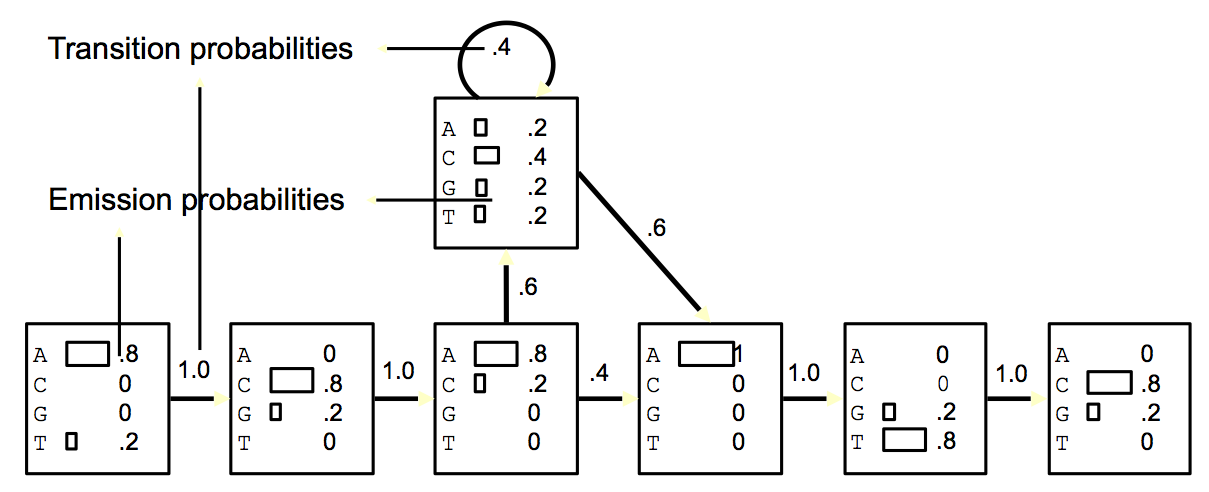
\includegraphics[width=.8\linewidth]{figs/HMM-example.png}}
\caption{Example of Hidden Markov Model}\label{fig:hmm}
\end{figure}

Each element $x_i$ of a sequence $x = x_1, ..., x_L$ is produced by state $\pi_i$. The path through the state machine is the sequence of states $\pi = \pi_1, ..., \pi_L$ that produced $x$.
Now given the sequence $x$ we can no longer identify the precise state from where each symbol $x_i$ was emitted, since several states could have produced it. This is why this MC is ``hidden''.

The HMM is characterized by {\em state transition} probabilities $a_{kl}$ and {\em symbol emission} probabilities $e_k$:
\begin{eqnarray}
a_{kl} & = & P(\pi_i=l \; | \; \pi_{i-1}=k) \label{eq:hmm:transition} \\
e_{k}(b) & = & P(x_i=b \; | \; \pi_i=k) \label{eq:hmm:emission}
\end{eqnarray}
%\begin{eqnarray}
%\boxed{a_{kl} = P(\pi_i=l \; | \; \pi_{i-1}=k)} \\
%\boxed{e_{k}(b) = P(x_i=b \; | \; \pi_i=k)}
%\end{eqnarray}
\begin{itemize}
\item The transition probability $a_{kl}$ is the probability that the current state $\pi_i$ is $l$ given that the previous state $\pi_{i-1}$ was $k$.
\item The emission probability $e_{k}(b)$ is the probability that symbol $b$ is emitted when we are in state $\pi_i=k$ (that is, given that the current state is $k$).
\end{itemize}

The HMM starts in state $\pi_0 = \alpha$ and ends in state $\pi_{L+1}=\omega$.

\subsubsection{Markov Property in HMM}

It is useful to rewrite the Markov property expressed by eq. \ref{eq:markovproperty} in the HMM context:
\begin{eqnarray}
P(\pi_i \; | \; \pi_{i-1}, ..., \pi_1) 
  = &  P(\pi_i \; | \; \pi_{i-1}) 
 & = \; a_{\pi_{i-1},\pi_i} \label{eq:markovhmm1}
\\
P(\pi_i \; | \; x_{i-1}, ..., x_1, \pi_{i-1}, ..., \pi_1) 
  = &  P(\pi_i \; | \; \pi_{i-1}) 
 & = \; a_{\pi_{i-1},\pi_i} \label{eq:markovhmm3}
\\
P(x_i \; | \; x_{i-1}, ..., x_1, \pi_{i}, \pi_{i-1}, ... , \pi_1) 
  = & P(x_i \; | \; \pi_{i}) 
 & = \; e_{\pi_i}(x_i) \label{eq:markovhmm2}
\end{eqnarray}

The probability of a path $\pi = \pi_0, \pi_1, ..., \pi_L, \pi_{L+1}$ can be calculated using the product rule and the Markov property from eq. (\ref{eq:markovhmm1}):
\begin{eqnarray}
P(\pi) & = & P(\pi_{L+1}, \pi_L, \pi_{L-1}, ..., \pi_1, \pi_0) \nonumber \\
     & = & P(\pi_{L+1}| \pi_L, ..., \pi_0) P(\pi_L, ..., \pi_0)  \nonumber \\
     & = & ...  \nonumber \\
     & = & P(\pi_{L+1}| \pi_L) P(\pi_L | \pi_{L-1}) ... P(\pi_1 | \pi_0) P(\pi_0) 
\Rightarrow  \nonumber
\end{eqnarray}
\begin{equation}
\boxed{P(\pi) = \prod_{i=0}^L P(\pi_{i+1}| \pi_i) = 
\prod_{i=0}^L a_{\pi_{i},\pi_{i+1}}}
\label{eq:probpi}
\end{equation}
for $P(\pi_0) = P(\pi_0=\alpha)=1$.

Therefore the probability of a path $\pi = \pi_0, \pi_1, ..., \pi_L, \pi_{L+1}$ is simply the product of the transition probabilities $a_{\pi_{i},\pi_{i+1}}$ along the path.

The joint probability of a sequence $x$ and a path $\pi$ is:
\begin{equation}
P(x,\pi) = P(x | \pi) P(\pi)
\label{eq:probxpi}
\end{equation}

$P(\pi)$ is given by eq. (\ref{eq:probpi}), so let's calculate $P(x | \pi)$,
using the product rule again, and the Markov assumption of eq. (\ref{eq:markovhmm2}):
\begin{eqnarray}
P(x | \pi) & = & 
P(x_L, x_{L-1}, ..., x_1 \; | \; \pi_{L+1}, \pi_L, \pi_{L-1}, ..., \pi_1, \pi_0)
\nonumber \\
  & = & 
P(x_L \; | \; x_{L-1}, ..., x_1, \pi_{L+1}, ..., \pi_0)
P(x_{L-1}, ..., x_1, \pi_{L+1}, ..., \pi_0)
\nonumber \\
  & = & 
P(x_L \; | \; \pi_L,)
P(x_{L-1} \; | \; x_{L-2}, ..., x_1, \pi_{L+1}, ..., \pi_0)
P(x_{L-2}, ..., x_1, \pi_{L+1}, ...,\pi_0)
\nonumber \\
  & = & 
P(x_L \; | \; \pi_L,) P(x_{L-1} \; | \; \pi_{L-1}) ... P(x_1 | \pi_1) P(x_0 | \pi_0) 
\Rightarrow  \nonumber
\end{eqnarray}
\begin{equation}
\boxed{P(x | \pi) = \prod_{i=0}^L P(x_{i} | \pi_i) = 
\prod_{i=0}^L e_{\pi_{i}}(x_i)}
\label{eq:probxgivenpi}
\end{equation}

Hence the probability of a sequence $x$ given a path $\pi$ is simply the product of the emission probabilities of the symbols $x_i$ of $x$ along the path $\pi$.

The joint probability $P(x,\pi)$ can now be obtained by substituting 
eqs. (\ref{eq:probpi}) and (\ref{eq:probxgivenpi}) in (\ref{eq:probxpi}):
\begin{equation}
P(x,\pi) = P(x | \pi) P(\pi) =
\prod_{i=0}^L e_{\pi_{i}}(x_i)
\prod_{i=0}^L a_{\pi_{i},\pi_{i+1}}
\Rightarrow
\end{equation}
\begin{equation}
\boxed{P(x,\pi) = \prod_{i=0}^L e_{\pi_{i}}(x_i) \; a_{\pi_{i},\pi_{i+1}}}
\label{eq:probxpi-final}
\end{equation}
which simply states that the joint probability of the sequence $x$ and the path $\pi$ is the product of the emission and transition probabilities along the path.

\subsection{Viterbi Algorithm}

Find the most probable path $\pi^*$ for a given sequence $x$:
\begin{equation}
\boxed{\pi^* = \argmax_{\pi} P(x,\pi)} \label{eq:viterbimax}
\end{equation}

Equation (\ref{eq:probxpi-final}) gives a way to calculate $P(x,\pi)$, however we don't have a path but would like to find the most probable one, without computing all possible paths, so eq. (\ref{eq:probxpi-final}) cannot be applied directly to compute eq. (\ref{eq:viterbimax}). A dynamic programming algorithm is used instead.

If we apply the product rule:
\begin{equation}
\pi^* = \argmax_{\pi} P(x,\pi) = \argmax_{\pi} P(\pi|x) P(x) 
= \argmax_{\pi} P(\pi|x)
\label{eq:viterbimax2}
\end{equation}
we see that the term $P(x)$ does not depend on $\pi$ hence does not influence the maximum and can be eliminated. \textcolor{red}{However starting with eq. (\ref{eq:viterbimax2}) instead of eq. (\ref{eq:viterbimax}) doesn't work to derive the Viterbi algorithm, because we get terms that we don't know how to compute. So we stick to eq. (\ref{eq:viterbimax}).}

Construct a partial solution up to position $\pi_i=k$:
\begin{equation}
v_k(i) = \max_{\pi_1,...\pi_{i-1}} P(x_1,...,x_i, \pi_1,...,\pi_{i-1}, \pi_i=k)
\end{equation}
for all possible $k$.

Use recursion to build the next step $v_l(i+1)$ of the solution as a function of the current step $v_k(i)$:
\begin{equation}
v_l(i+1) = \max_{\pi_1,...\pi_{i}=k} P(x_1,...,x_{i+1}, \pi_1,...\pi_{i}=k, \pi_{i+1}=l)
\end{equation}
where $k$ is the optimum state chosen in the maximization step $v_k(i)$, and $l$ is the new optimum to be determined for the next step $v_l(i+1)$.

Use the product rule and the Markov property to break down $v_l(i+1)$ into known elements that can be computed:
\begin{eqnarray}
v_l(i+1)
& = &
\max_{\pi_1,...\pi_{i}=k}
P(x_1,...,x_{i+1}, \pi_1,...\pi_{i}=k, \pi_{i+1}=l)
\nonumber \\
& = &
\max_{\pi_1,...\pi_{i}=k}
P(x_{i+1} | x_1, ..., x_i, \pi_1,...\pi_{i}=k, \pi_{i+1}=l)
P(x_1, ..., x_i, \pi_1,...\pi_{i}=k, \pi_{i+1}=l)
\nonumber \\
& = &
\max_{\pi_1,...\pi_{i}=k}
P(x_{i+1} | \pi_{i+1}=l)
P(\pi_{i+1}=l | x_1, ..., x_i, \pi_1,...\pi_{i}=k) 
P(x_1, ..., x_i, \pi_1,...\pi_{i}=k)
\nonumber \\
& = &
\max_{\pi_1,...\pi_{i}=k}
P(x_{i+1} | \pi_{i+1}=l)
P(\pi_{i+1}=l | \pi_{i}=k)
P(x_1, ..., x_i, \pi_1,...\pi_{i}=k)
\nonumber \\
& = &
\max_{\pi_1,...\pi_{i}=k}
e_l(x_{i+1}) \;
a_{kl} \;
P(x_1, ..., x_i, \pi_1,...\pi_{i}=k)
\end{eqnarray}

Now break the maximization step in two parts: maximize over $\pi_1,...,\pi_{i-1}$ and then maximize over $\pi_i=k$:
\begin{equation}
v_l(i+1) =
\max_{\pi_{i}=k} \quad
\max_{\pi_1,...\pi_{i-1}}
e_l(x_{i+1}) \;
a_{kl} \;
P(x_1, ..., x_i, \pi_1,...\pi_{i}=k)
\end{equation}

The term $e_l(x_{i+1})$ does not depend on $\pi_1,...,\pi_i$ so can be take out of both max functions. Moreover the term $a_{kl}$ does not depend on $\pi_1,...\pi_{i-1}$ hence can be taken out of the inner max:
\begin{equation}
v_l(i+1) =
e_l(x_{i+1}) \;
\max_{\pi_{i}=k} \left(
a_{kl} \;
\max_{\pi_1,...\pi_{i-1}}
P(x_1, ..., x_i, \pi_1,...\pi_{i}=k)
\right)
\label{eq:viterbimaxmax}
\end{equation}

Now we recognize the last max term of eq. (\ref{eq:viterbimaxmax}) above as $v_k(i)$, arriving at the {\bf Viterbi recursion} formula:
\begin{equation}
\boxed{v_l(i+1) = e_l(x_{i+1}) \; \max_{\pi_{i}=k} \; ( \; a_{kl} \; v_k(i) \; )}
\label{eq:viterbi}
\end{equation}

Viterbi finds the most probable path $\pi^*$, but since the number of possible paths is usually huge, the probability of $\pi^*$ might actually be very small (even if bigger than the other even smaller probabilities for the other paths), so in practice the ``optimal'' path $\pi^*$ is of little use.



\subsection{Forward Algorithm}
\label{sec:fwdalg}

The forward algorithm computes the probability of a sequence $x$ of length $L$, $x = x_1, ... x_L$, for all possible paths $\pi$.
\begin{equation}
\boxed{P(x) = \sum_\pi P(x, \pi)}
\end{equation}

As in the Viterbi case, we don't want to use eq. (\ref{eq:probxpi-final}) directly since it would require enumerating all possible paths. Dynamic programming is again the solution here.

Start with a partial solution $f_k(i)$, the probability of subsequence $x_1,... , x_i$ when $x_i$ is emitted by state $k$:
\begin{equation}
f_k(i) = P(x_1,...,x_i, \pi_i = k)
\label{eq:fwdfki}
\end{equation}
for all possible combinations of $\pi_1,... \pi_{i-1}$ (these $\pi_1,... \pi_{i-1}$ are not given, hence they do not appear in eq. (\ref{eq:fwdfki})).

Define the next step $f_l(i+1)$:
\begin{equation}
f_l(i+1) = P(x_1,...,x_{i+1}, \pi_{i+1} = l)
\label{eq:fwdfli1}
\end{equation}

We do not know $\pi_i = k$, so we must use marginalization to sum over all possible values of $k$:
\begin{equation}
f_l(i+1) = \sum_{k=1}^K P(x_1,..., x_i, x_{i+1}, \pi_i=k, \pi_{i+1} = l)
\label{eq:fwdfli2}
\end{equation}
where $K$ is the number of states in the HMM.

Apply the product rule to eq. (\ref{eq:fwdfli2}) with the goal to isolate $f_k(i)$, so we pick $x_{i+1}$ first:
\begin{equation}
f_l(i+1) = \sum_{k=1}^K 
P(x_{i+1} | x_1,..., x_i,  \pi_i=k, \pi_{i+1} = l)
P(x_1,..., x_i,  \pi_i=k, \pi_{i+1} = l)
\label{eq:fwdfli3}
\end{equation}

Now use the Markov property:
\begin{equation}
f_l(i+1) = \sum_{k=1}^K 
P(x_{i+1} | \pi_{i+1} = l)
P(x_1,..., x_i,  \pi_i=k, \pi_{i+1} = l)
\label{eq:fwdfli4}
\end{equation}

Apply the product rule again, now picking $\pi_{i+1} = l$ to make $f_k(i)$ appear:
\begin{equation}
f_l(i+1) = \sum_{k=1}^K 
P(x_{i+1} | \pi_{i+1} = l)
P(\pi_{i+1} = l | x_1,..., x_i,  \pi_i=k)
P(x_1,..., x_i,  \pi_i=k)
\label{eq:fwdfli5}
\end{equation}

Use the Markov property:
\begin{equation}
f_l(i+1) = \sum_{k=1}^K 
P(x_{i+1} \; | \; \pi_{i+1} = l) \;
P(\pi_{i+1} = l \; | \; \pi_i=k) \;
P(x_1,..., x_i, \pi_i=k)
\label{eq:fwdfli6}
\end{equation}

We now recognize the terms of eq. (\ref{eq:fwdfli6}) as $e_l(x_{i+1})$, $a_{kl}$, and $f_k(i)$, respectively:
\begin{equation}
f_l(i+1) = \sum_{k=1}^K e_l(x_{i+1}) \; a_{kl} \; f_k(i)
\label{eq:fwdfli7}
\end{equation}

The term $e_l(x_{i+1})$ does not depend on $k$, hence can be taken out of the sum, leading to the final recursion equation for the forward algorithm:
\begin{equation}
\boxed{f_l(i+1) = e_l(x_{i+1}) \sum_{k=1}^K a_{kl} \; f_k(i) }
\label{eq:fwdrecursion}
\end{equation}
%where $S$ is the set of states of the HMM,
%e.g. $S = \{ \alpha, E, I, W, \omega \}$.

\subsection{Backward Algorithm}

This algorithm computes the probability that state $\pi_i = k$ was the one that generated symbol $x_i$, given the entire sequence $x = x_1, ... x_L$:
\begin{equation}
\boxed{P(\pi_i = k | x) = P(\pi_i = k \; | \; x_1, ... x_L)}
\label{eq:bk0}
\end{equation}

Note that $P(\pi_i = k | x) \ne P(x_i | \pi_i = k)$:
\begin{itemize}
\item $P(\pi_i = k | x)$ is the probability that state $k$, out of all possible states of the HMM, was the one responsible for generating $x_i$ in $x$ (but we don't know for sure which state actually generated $x_i$);
\item $P(x_i | \pi_i = k) = e_k(x_i)$ is the emission probability of $x_i$ from state $k$ once we {\em know} that we are in state $k$ (state $k$ is {\em given}).
\end{itemize}

Using the product rule:
\begin{eqnarray}
P(x, \pi_i = k) & = & P(\pi_i = k | x) P(x) \Rightarrow \\
P(\pi_i = k | x) & = & \frac{P(x, \pi_i = k)}{P(x)}
\label{eq:bk3}
\end{eqnarray}

The denominator $P(x)$ can be computed by the foward algorithm.
Let's then compute the numerator $P(x, \pi_i = k)$ using the product rule and the Markov property:
\begin{eqnarray}
P(x, \pi_i = k) 
& = & P(x_1, ..., x_i, x_{i+1}, ..., x_L, \pi_i=k) \nonumber \\
& = & P(x_1, ..., x_i, \pi_i=k, x_{i+1}, ..., x_L) \nonumber \\
& = & 
P(x_{i+1}, ..., x_L | x_1, ..., x_i, \pi_i=k)
P(x_1, ..., x_i, \pi_i=k) \nonumber \\
& = & 
P(x_{i+1}, ..., x_L | \pi_i=k)
P(x_1, ..., x_i, \pi_i=k)
\label{eq:bk1}
\end{eqnarray}

We recognize the last term of eq. (\ref{eq:bk1}) as $f_k(i)=P(x_1, ..., x_i, \pi_i=k)$. Call the remaining term $b_k(i)$:
\begin{equation}
b_k(i) = P(x_{i+1}, ..., x_L | \pi_i=k)
\label{eq:bki}
\end{equation}

Equation (\ref{eq:bk1})  then becomes:
\begin{equation}
P(x, \pi_i = k) = f_k(i) b_i(i)
\label{eq:bk2}
\end{equation}

\textcolor{red}{Note that we cannot eliminate $\pi_i=k$ from eqs.
(\ref{eq:bk1}) or (\ref{eq:bki})
using the Markov property: even though $x_{i+1}, ..., x_L$ do not depend directly on $\pi_i=k$, the term $\pi_{i+i}$ upon which $x_{i+1}$ depends is unknown, and $\pi_{i+i}$ on its turn depends on $\pi_i$, hence we must leave $\pi_i=k$ there. If we knew $\pi_{i+i}$, then we could have scratched out $\pi_i=k$.}

We must now build a recursion from backwards to compute $b_k(i)$:
\begin{equation}
b_l(i+1) = P(x_{i+2}, ..., x_L | \pi_{i+1}=l)
\label{eq:bkli1}
\end{equation}

We don't know $\pi_{i+1}=l$, hence we must use marginalization to compute all possibilities for it:
\begin{equation}
b_k(i) = \sum_{l=1}^K P(x_{i+1}, x_{i+2}, ..., x_L, \pi_{i+1}=l | \pi_i=k)
\end{equation}
\textcolor{red}{Since $\pi_{i+1}=l$ is unknown, hence not given, it appears at the front part of the probability rule, not at the tail (the ``given'' part)}.

Now apply the product rule $P(A,B|D) = P(A|B,D) P(B|D)$ with: \\
$A \leftarrow (x_{i+1}, x_{i+2}, ..., x_L)$,
$B \leftarrow (\pi_{i+1}=l)$,
$D \leftarrow (\pi_i=k)$:
%
\begin{equation}
b_k(i) = \sum_{l=1}^K P(x_{i+1}, x_{i+2}, ..., x_L \; | \; \pi_{i+1}=l, \pi_i=k) \;
                         P(\pi_{i+1}=l \; | \; \pi_i=k)
\end{equation}

We recognize the last term of the above equation as $a_{kl}$. Moreover now we can eliminate $\pi_i=k$ from the first term using the Markov property, since $\pi_{i+1}=l$ is given there:
\begin{equation}
b_k(i) = \sum_{l=1}^K P(x_{i+1}, x_{i+2}, ..., x_L \; | \; \pi_{i+1}=l) \; a_{kl}
\end{equation}

Now apply the product rule $P(A,B|D) = P(A|B,D) P(B|D)$ again with: \\
$A \leftarrow (x_{i+1})$,
$B \leftarrow (x_{i+2}, ..., x_L)$,
$D \leftarrow (\pi_{i+1}=l)$:
%
\begin{eqnarray}
b_k(i) & = & \sum_{l=1}^K 
P(x_{i+1} \; | \; x_{i+2}, ..., x_L, \pi_{i+1}=l)  \;
P(x_{i+2}, ..., x_L \; | \; \pi_{i+1}=l) 
\; a_{kl}
\nonumber \\
& = &  \sum_{l=1}^K 
P(x_{i+1} \; | \; \pi_{i+1}=l) \;
b_l(i+1)
\; a_{kl}
\Rightarrow
\nonumber
\end{eqnarray}
%
\begin{equation}
\boxed{b_k(i) =  \sum_{l=1}^K  e_l(x_{i+1}) \; b_l(i+1) \; a_{kl}}
\end{equation}
which is the final recursion formula for $b_k(i)$.

Now that we know how to compute $b_k(i)$, we can go back to eqs. (\ref{eq:bk3}) and (\ref{eq:bk2}) to tackle our original goal to compute $P(\pi_i = k | x)$:

\begin{equation}
\boxed{P(\pi_i = k | x) = \frac{P(x, \pi_i = k)}{P(x)} 
                        = \frac{f_k(i) \; b_k(i)}{P(x)}}
\end{equation}

Now all the terms $f_k(i)$, $b_k(i)$, and $P(x)$ can be computed.

\subsection{Posterior decoding \textcolor{green}{sl 20}}

Instead of using the most probable path (Viterbi), use the path of the most probable states:
\begin{equation}
\hat{\pi}_i = \argmax_k P(\pi_i = k | x)
\end{equation}
where $P(\pi_i = k | x)$ can be computed by the backward algorithm. Caution however because the path $\hat{\pi}_i$ can be illegal!!

\subsection{Parameter estimation with known paths \textcolor{green}{sl 25}}

Given a training set $\mathcal{D}$ of $N$ sequences $x^1, ... x^N$: 
$\mathcal{D} = \{ x^1, ... x^N \}$,
we would like to find the set of parameters $\theta$ that maximize the likelihood of seeing these sequences: $\argmax_\theta P(x|\theta)$.

Score the model using the log likelihood of the parameters $\theta$ given the training data:
\begin{equation}
\text{Score}(\mathcal{D},\theta) = \log P(x^1, ... , x^N | \theta) 
                           = \sum_{j=1}^N \log P(x^j | \theta)
\end{equation}

The parameters in this case are the transition and emission probabilities $\theta = \{ a_{kl}, e_k(b) \}$ for all states and symbols. With known paths, it suffices to walk along these paths for all training sequences, and to count how often a transition to state $l$ is used from state $k$ ($A_{kl}$), and how often a symbol $b$ is produced from state $k$ ($E_k(b)$. The probabilities $a_{kl}$ can then be obtained by ML estimation as we saw in section \ref{sec:mlintuitive}
\begin{eqnarray}
a_{kl} & = & \frac{A_{kl}}{\sum_{l'} A_{kl'}}
\label{eq:akl}
\\
e_k(b) & = & \frac{E_k(b)}{\sum_{b'} E_k(b')}
\label{eq:ekb}
\end{eqnarray}
or better, by using pseudocounts as explained in section \ref{sec:pseudocounts}: in this case, $A_{kl}$ and $E_k(b)$ can include the pseudocounts.

\subsection{Parameter estimation with unknown paths \textcolor{green}{sl 27}}

When the paths $\pi$ are unknown, we cannot simply count the frequencies as we did in the previous section, because we don't know where to go in the HMM, given just the sequences $x$. The solution here is to estimate the parameters and the paths using an iterative method, via progressive refinement from a initially coarse solution. Two algorithms can take care of this: Viterbi training and Baum-Welch training.

\subsubsection{Viterbi training}

Viterbi training makes use of the Viterbi algorithm to compute the most probable path $\pi^*$ for each traning sequence, given a coarse initial assignment of $\theta = \{ a_{kl}, e_k(b) \}$ (for instance, initially all states and all transitions are equally probable). These paths are then used to estimate new frequencies via counting, using eqs. (\ref{eq:akl}) and (\ref{eq:ekb}). These new frequencies are then used to obtain new optimum paths, and so on. This process is repeated using the new frequencies and the optimum paths from the previous iteration to refine the frequencies and paths for the next iteration, until convergence, leading to a simultaneous estimation of the optimum path and the optimum parameters:
%
\begin{equation}
x,\theta^0 \rightarrow \text{Viterbi} \rightarrow x, \pi \rightarrow 
\text{count} \rightarrow x,\theta^1 \rightarrow \text{Viterbi} 
\rightarrow ... \rightarrow x,\pi^*, \theta^*
\end{equation}

The algorithm is guaranteed to converge to a set of parameters such that the same path results from the same parameters, so at some point things stop changing, that is, the algorithm converges.
However it is too greedy (takes the most probable path at each step, which might ignore a vast amount of good paths). Moreover it does not compute the maximum likelihood estimate for the parameters:
\begin{equation}
\theta^* \ne \argmax_\theta P(x_1, ..., x_N|\theta)
\end{equation}
where $\theta^*$ is the optimum $\theta$ found by Viterbi training, and $x_1,...,x_N$ are the sequences from the training set.

\subsubsection{Baum-Welch training \textcolor{green}{sl 28}}
\label{sec:baumwelch}

Instead of taking only the most probable path at each step and ignoring all the others as done by Viterbi training, the Baum-Welch algorithm estimates the parameters $\theta = \{ a_{kl}, e_k(b) \}$ by calculating the {\em expected} number of times each transition or emission is used, for all possible paths. Of course, it must do this without enumerating all possible paths explicitly, which can be achieved by using the forward and the backward algorithms.

Remember that the forward algorithm computes the probability of a sequence for all possible paths, and the backward algorithm computes the probability that a particular state was the one that produced a particular symbol in a sequence.

Moreover in section \ref{sec:fwdalg} we saw that the forward algorithm is computed using the existing parameters $\theta = \{ a_{kl}, e_k(b) \}$ that were then given, but that we are now going go estimate. So actually the forward algorithm computes $P(x|\theta)$ which is the likelihood of the data $x$ given the parameters $\theta$. The partial solution $f_k(i)$ then becomes:
%
\begin{equation}
f_k(i) = P(x_1,...,x_i, \pi_i = k | \theta)
\label{eq:fwdfki:bw}
\end{equation}

Similarly, the backward algorithm computes $P(\pi_i = k | x, \theta)$, and its
partial solution is:
\begin{equation}
b_l(i+1) = P(x_{i+2}, ..., x_L | \pi_{i+1}=l, \theta)
\label{eq:bkli1:bw}
\end{equation}

The probability that transition $k \rightarrow l$ is used in a particular sequence $x$ is given by:
\begin{equation}
P(\pi_i = k, \pi_{i+1} = l | x, \theta) 
=
\frac{P(\pi_i = k, \pi_{i+1} = l, x | \theta)}{P(x|\theta)}
\end{equation}

Initially we don't know any parameters, so we set $\theta = \theta^0$ to their pseudocount values.
$P(x|\theta)$ can be computed by the forward algorithm so we focus on the other term:
%
\begin{eqnarray}
P(\pi_i = k, \pi_{i+1} = l, x | \theta) & = &
P(x_1, ..., x_L, \pi_i = k, \pi_{i+1} = l | \theta) 
\\ 
& = &
P(x_1, ..., x_i, \pi_i = k, \pi_{i+1} = l, x_{i+1}, ..., x_L | \theta) 
\\
& = &
P(x_{i+1}, ..., x_L, \pi_{i+1} = l | x_1, ..., x_i, \pi_i = k, \theta)
\nonumber
\\
&&
P(x_1, ..., x_i, \pi_i = k | \theta)
\end{eqnarray}
We recognize the last line as $f_k(i)=P(x_1, ..., x_i, \pi_i = k | \theta)$, so let's develop the other one:
%
\begin{eqnarray}
&&
P(x_{i+1}, ..., x_L, \pi_{i+1} = l | x_1, ..., x_i, \pi_i = k, \theta)
=
\nonumber
\\
&&
P(x_{i+1}, ..., x_L, \pi_{i+1} = l | \pi_i = k, \theta)
=
\nonumber
\\
&&
P(x_{i+1}| x_{i+2}, ..., x_L, \pi_{i+1} = l, \pi_i = k, \theta)
P(x_{i+2}, ..., x_L, \pi_{i+1} = l | \pi_i = k, \theta)
=
\nonumber
\\
&&
P(x_{i+1}| \pi_{i+1} = l, \theta)
P(x_{i+2}, ..., x_L | \pi_{i+1} = l , \pi_i = k, \theta)
P(\pi_{i+1} = l | \pi_i = k, \theta)
=
\nonumber
\\
&&
P(x_{i+1}| \pi_{i+1} = l, \theta)
P(x_{i+2}, ..., x_L | \pi_{i+1} = l , \theta)
P(\pi_{i+1} = l | \pi_i = k, \theta)
=
\nonumber
\\
&&
e_l(x_{i+1}) b_l(i+1) a_{kl}
\end{eqnarray}

Combining all together we get:
\begin{equation}
P(\pi_i = k, \pi_{i+1} = l | x, \theta) = 
\frac{a_{kl} \; e_l(x_{i+1}) \; f_k(i) \; b_l(i+1)}{P(x|\theta)}
\label{eq:pakl:bw}
\end{equation}
%
All these terms can be computed using the forward and backward algorithms, using the estmations of parameters from the previous iteration.

The expected number of times that transition $a_{kl}$ is used can be estimated by summing eq. (\ref{eq:pakl:bw}) for all positions in all training sequences:
\begin{eqnarray}
A_{kl} & = &
\sum_{j=1}^N \sum_{i=1}^L
P(\pi_i = k, \pi_{i+1} = l | x_i^j, \theta)
\\
& = &
\sum_{j=1}^N \frac{1}{P(x^j|\theta)}
\sum_{i=1}^L
a_{kl} \; e_l(x_{i+1}^j) \; f_k^j(i) \; b_l^j(i+1)
\end{eqnarray}

The expected emission count is obtained in a similar way, by summing over all positions $i$ in all sequences $x^j$ where the symbol $x_i^j$ at position $i$ in sequence $j$ is $b$:
% PENDING DERIVATION
\begin{eqnarray}
E_k(b) & = & \sum_j \sum_{i | x_i^j = b} P(\pi_i=k | x^j, \theta)
\\
& = & \sum_j \frac{1}{P(x^j|\theta)}
\sum_{i | x_i^j = b}
f_k^j(i) \; b_k^j(i)
\end{eqnarray}

Using these expected counts, new transition and emission parameters can be estimated for use in the next iteration, using eqs. (\ref{eq:akl}) and (\ref{eq:ekb}), repeated here for convenience:
\begin{eqnarray}
a_{kl} & = & \frac{A_{kl}}{\sum_{l'} A_{kl'}}
\label{eq:akl-bis}
\\
e_k(b) & = & \frac{E_k(b)}{\sum_{b'} E_k(b')}
\label{eq:ekb-bis}
\end{eqnarray}

The resulting algorithm is shown in figure \ref{fig:baumwelch}. At each iteration, the Baum-Welch algorithm improves the likelihood estimate of the parameters, in contrast with Viterbi training.
We will see in section \ref{sec:em} that Baum-Welch training is a special case of Expectation Maximization (EM) algorithm.

\begin{figure}[!htb]
\centerline{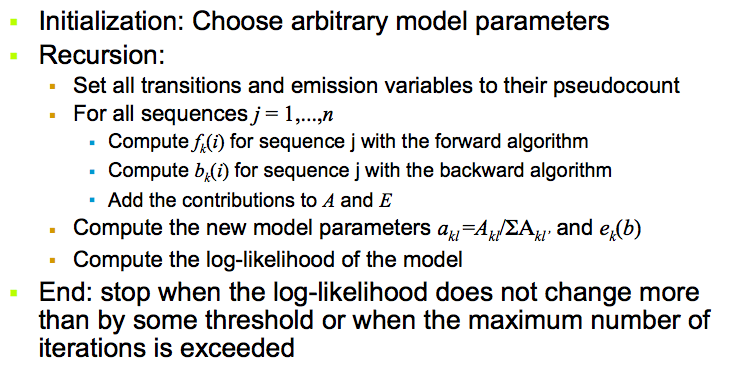
\includegraphics[width=.6\linewidth]{figs/BaumWelch.png}}
\caption{The Baum-Welch training algorithm}\label{fig:baumwelch}
\end{figure}

A major limitation of Baum-Welch training is that it consumes a lot of data to estimate the parameters from scratch (when no prior knowledge is available): thousands of observations might be needed to produce a good model, and then thousands more to reduce the error by a factor 10. However, prior knowledge can greatly reduce the number of observations needed to get a sufficiently good estimation of parameters.

Another issue is the problem of numerical instability due to the product of small probabilities: simply taking log scale works well for Viterbi, but doesn't work well for the forward algorithm, because we get logs of sums, which are not so nice.
The solution is to take approximations of algorithms, or define new variables that are in log-like scale.


%---------------------------------------------------------------------------

\subsection{HMM Applications}

\subsubsection{Profile HMMs}

\subsubsection{Gene Finding}

predict the location of genes; often combined with homology search.

analysis of codon bias

GENSCAN: gene prediction using Hidden Semi-Markov Models

semi-markov chain:
before moving to next state, can stay there for a certain period of time; number of discrete time steps drawn from a distribution:
draw from that discrete distr to decide if you stay in that state or move on

Hidden Semi-Markov:
enter state: each state may be a quite complex model:
can put a whole HMM inside the state, and from this HMM you can generate a small subsequence before moving to the next state

